% !TEX root = main.tex

\section{XXX Model}
To address the above-described challenges, we propose XXX. Fig. \ref{fig:architecture} depicts the overall architecture of our XXX model. Correlating to the three phases introduced in section \ref{subsec:methodology}, we explain our model in following three aspects, input, rGCN layers and prediction.

\begin{figure}[htbp]
	\centering
	\label{fig:architecture}
	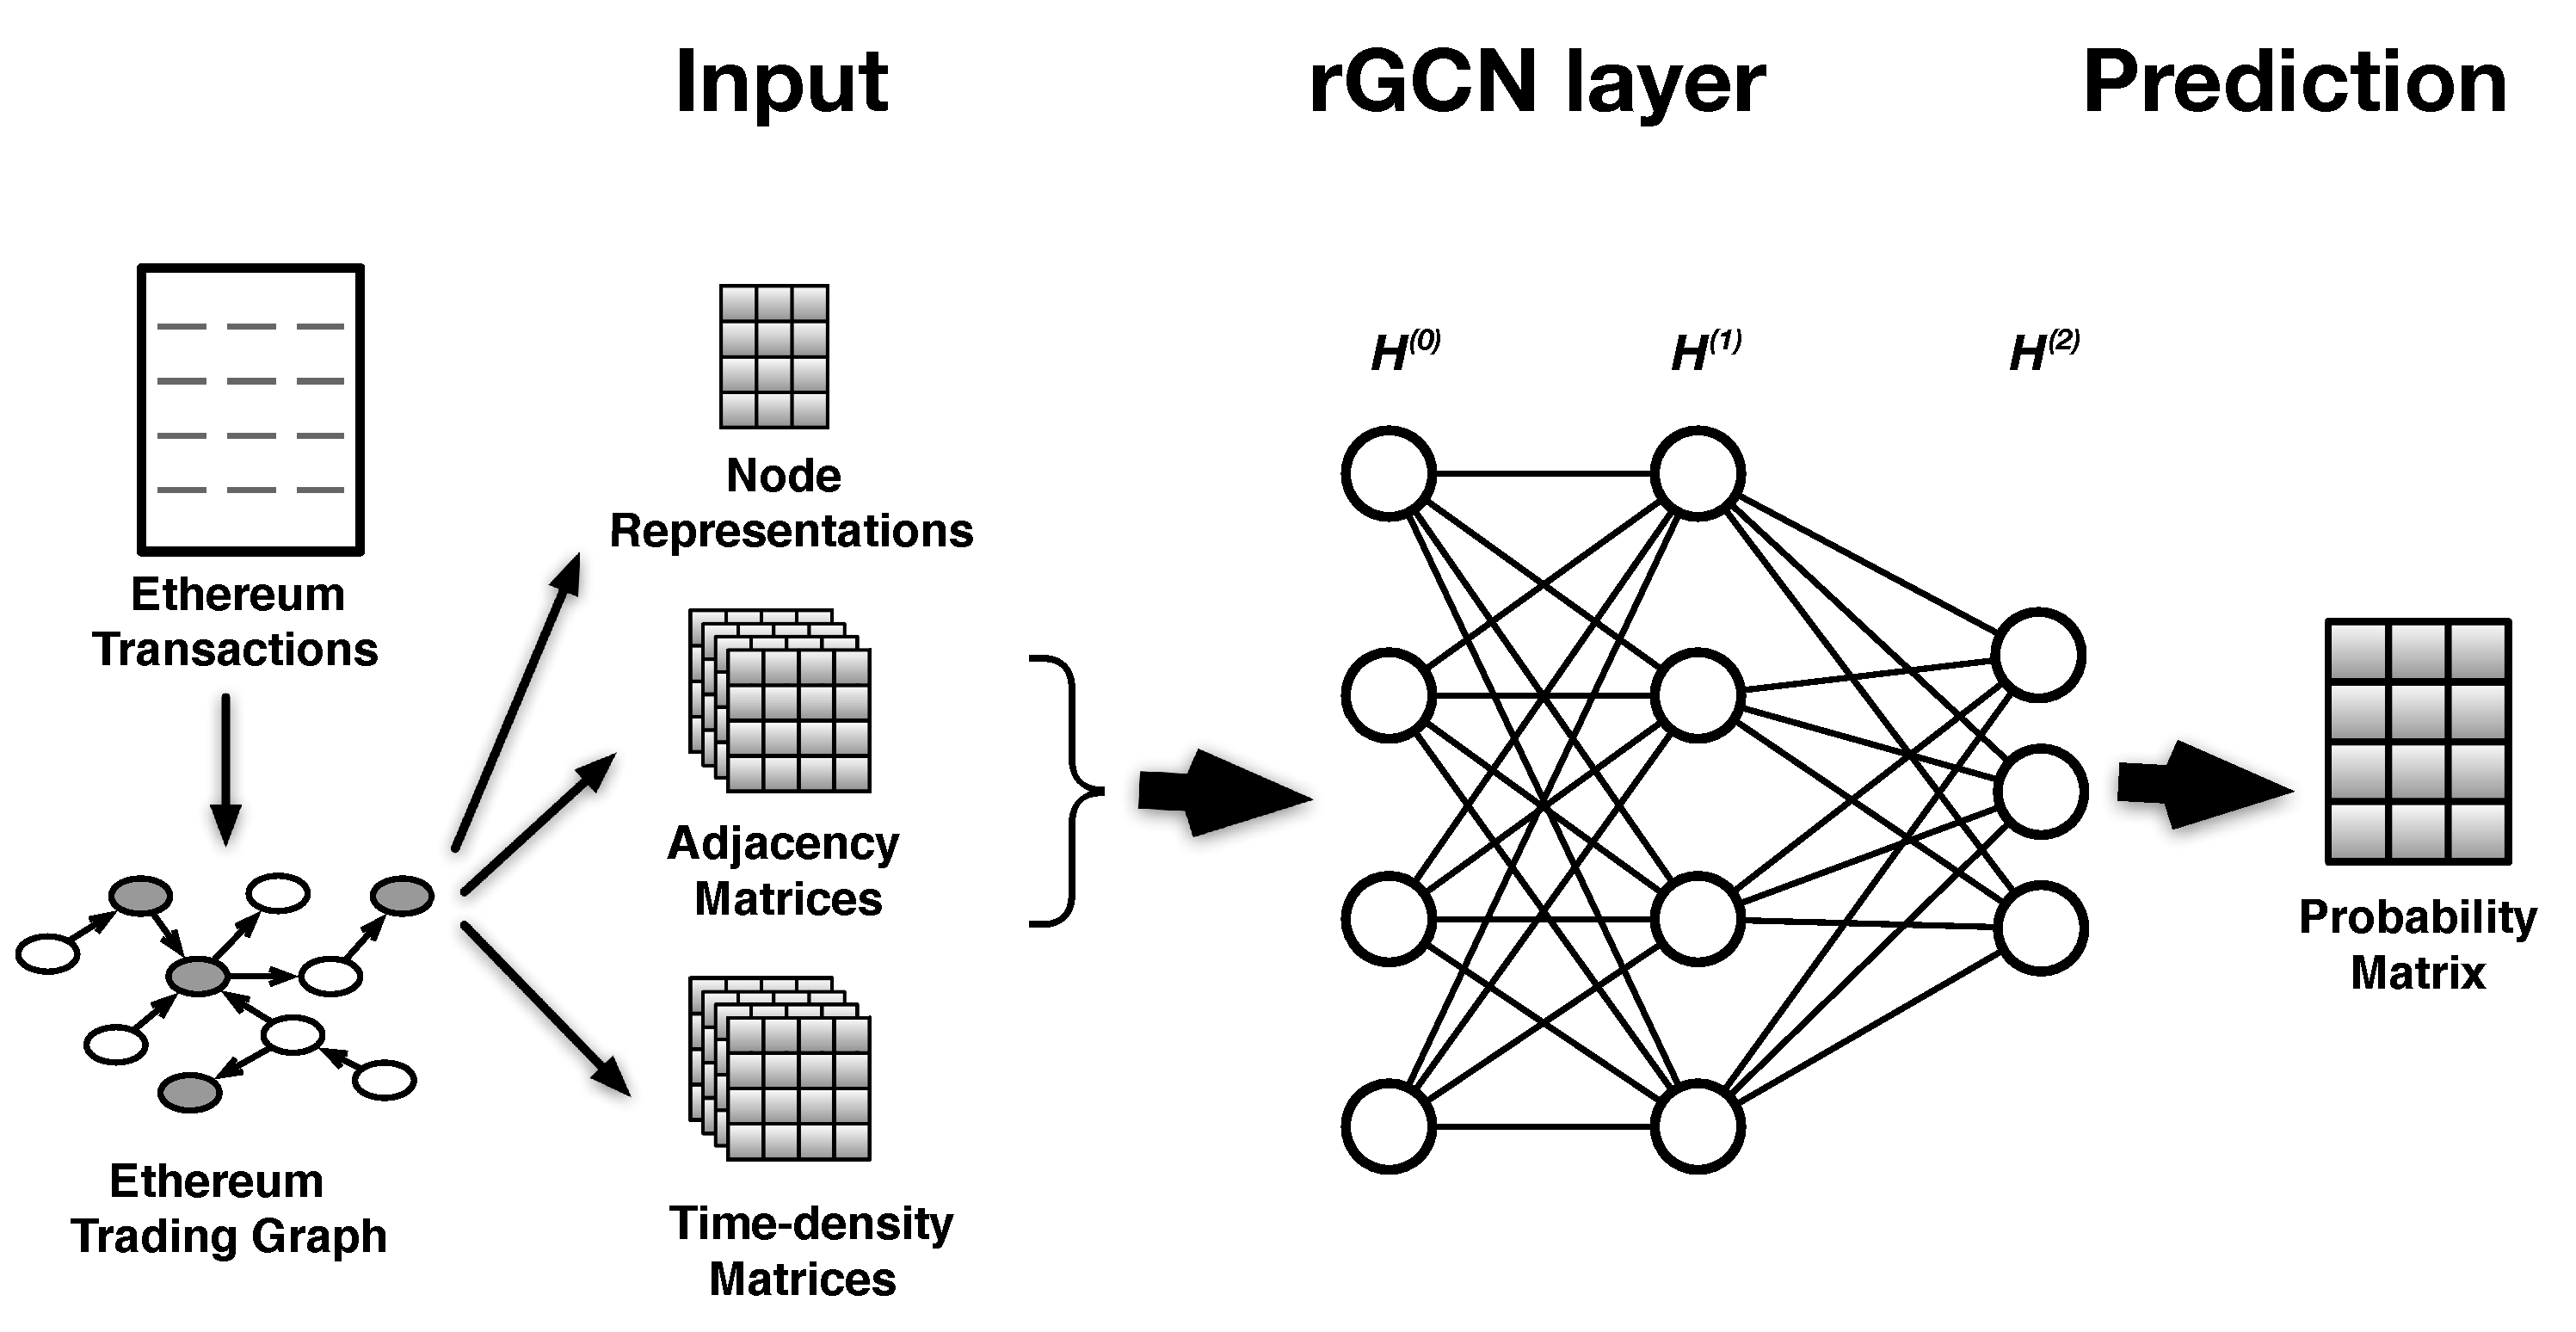
\includegraphics[width=3.5in]{fig/architecture.eps}
	\caption{overall architecture.}
	%\caption{Example of a figure caption.}
\end{figure}


\subsection{Input}
\label{sec:input}
 The input consists of three parts: a node feature matrix that captures the structural information of nodes, a list of time-density matrices that represent transaction intensiveness between each pair of nodes, and a list of adjacency matrices which describe different relations.

\textbf{Node representations.} We use a feature matrix $X \in \mathbb{R}^{N \times d}$ to encode the overall structural information of each node. The $d$ terms include node connection features such as in-degree, out-degree, weighted degree, eccentricity, clustering coefficient. Besides, the account type (EOA or SC) is also considered.   

These features help the following layers to pay attention to structural similarity between nodes.

\textbf{Node relations.} We divide the raw ETG into different graphs and capture the relations of graph neighboring nodes using adjacency matrices. The list of adjacency matrices, $\{A^1,A^2,...,A^R|A^i\in \mathbb{R}^{N \times N}\}$ describes the $R$ relations among $N$ nodes in ETG.

The $R$ relations are constructed from three aspects. The first one consists the 4 types of forward transactions discussed before: CALLs with ETH, CALLs without ETH, CREATIONs and REWARDs, which represent the relations of ETH transferring, smart contract invocation, smart contract deployment and mining reward. The second part includes 4 reverse relations in order to pass information from the opposite direction. Last a self loop as a special relation type is included to \textcolor{red}{TBA}.

\textcolor{red}{Specially, the adjacency matrices are modified to preserve the asymmetric proximity of ETG, which will be addressed in detail later.}




\textbf{Time-density matrices.} We find that the relationship between a pair of nodes grow more closely when their transactions happen intensively, so we propose time-density to merge transactions.

 Correlated to the adjacency matrices, a list of time-density matrices $\{K^1,K^2,...,K^R|K^i\in \mathbb{R}^{N \times N}\}$ describes the concentration of relations. The time-density matrix of each relation $r$ between node $v_i$ and $v_j$ is computed as%Equation \ref{eq:time}
\begin{equation}
k_{ij}^r=g(var(\texttt{bh}_{ij}^r))
\label{eq:time}
\end{equation}

where $\texttt{bn}_{ij}^{r}$ is the block height set of relation $r$ between node $v_i$ and $v_j$. And $g(\cdot)$ is the function of \textcolor{red}{TBA} which can be logarithmic function.


\subsection{GCN layers}
\label{sec:rGCN layers}
 We feed the input into two rGCN layers (Section \ref{sec:rGCN layers}), as a trade-off between preserving high-order proximities and introducing noise.

The input to rGCN $l$-th layer is defined as $H^{(l)}={h_1^{(l)},h_2^{(l)},...,h_N^{(l)}|h_i^{(l)}\in \mathbb{R}^{N \times d^{(l)}}}$.

In raw rGCN model, the propagation model can be expressed as

\begin{equation}
h_i^{(l+1)}=\delta(\sum_{r\in R} \sum_{j \in N_i^r} \frac{1}{c_{i,r}}W_r^{(l)}h_j^{(l)}+W_0^{(l)}h_i^{(l)})
\label{eq:rgcn}
\end{equation}

where $r \in R$ represents a kind of relation, $N_i^r$ denotes the set of neighbor indices of node $v_i$ under relation $r$, and $c_{i,r}=\frac{1}{|N_i^r|}$. Single self-connection is also introduced as a special relation type to each node. %compared with Eq.\ref{eq:gcn}The node feature $h_i$ is updated as:

We modified the forward updating process as 
\begin{equation}
h_i^{(l+1)}=\delta(\sum_{r\in R} \sum_{j \in N_i^r} \frac{\tau_{ij}^r}{\hat c_{i,r}}W_r^{(l)}h_j^{(l)})
\end{equation}
where $\tau_{ij}^r$ is the time-density of transactions from node $v_i$ to $v_j$. 

The coefficient $\hat c_{i,r}$ is computed as:
\begin{equation}
\hat c_{i,r}=\frac{1}{d_i^r\cdot N_i^r}
\end{equation}
where $d_i^r=\sum_{j}A^r_{ij}$, preserving the asymmetric proximity.


\subsection{Prediction and Training}
The output of the last layer indicates the probability that each point being assigned to each class.

The output of the last rGCN layer is regarded as a probability matrix $P=\{p_1,p_2,...,p_N|p_i\in \mathbb{R}^{N \times m}\}$, where $p_i=\{p_{i,1},p_{i,2},...,p_{i,m}\}$ describes the probability of classifying node $v_i$ into $m$ categories. 

We utilize the cross-entropy loss function as the training objective:
\begin{equation}
L=-\sum_{i=1}^T\sum_{j=1}^m y_{i,j}\log p_{i,j}+\lambda ||\theta||^2
\end{equation}
where $T$ is the number of training samples, $y_{i,j}$ is the true probability of node $v_i$ belonging to category $j$. $\theta$ is the set of all parameters and $\lambda$ is the coefficient for $L_2$  regularization.
